\section{Metodología}

\subsection{Materiales y Herramientas}

\begin{itemize}
    \item Microcontrolador ATmega328P (Arduino Uno)
    \item Sensor LDR y LED RGB
    \item Servomotor SG90
    \item Teclado matricial 4x4
    \item Pantalla LCD 16x2 con interfaz I2C
    \item Buzzers piezoeléctricos (activo y pasivo)
    \item Tira LED WS2812
    \item Resistencias, cables, protoboard
    \item Software: Microchip Studio, Proteus / PicSimLab, Python (para generación de secuencias del plotter)
\end{itemize}

\subsection{Procedimiento general}
Se dividió el sistema en cuatro módulos independientes (Plotter, Colores, Piano y Cerradura).

\subsubsection{\textbf{Plotter}}

    \vspace{1em}
    
\subsubsection{\textbf{Colores}}
    El proceso de reconocimiento de colores se fundamenta en la descomposición de cada color en sus componentes primarias dentro del modelo RGB (\textit{Red}, \textit{Green}, \textit{Blue}). Un color puede representarse como la combinación ponderada de estas tres intensidades, lo que permite su descripción en un espacio tridimensional.  

    \vspace{1em}

    Sin embargo, el sensor fotoresistivo (LDR, \textit{Light Dependent Resistor}) utilizado en el sistema no distingue de forma individual las componentes cromáticas del espectro visible; únicamente mide la intensidad total de luz reflejada sobre su superficie. Si la iluminación se realiza con luz blanca, el sensor solo entrega una lectura proporcional a la cantidad total de luz reflejada, sin discriminar su composición espectral. Este fenómeno equivale a una percepción en escala de grises, dificultando la identificación precisa de colores.

    \vspace{1em}

    Para resolver esta limitación, se empleó un diodo emisor de luz RGB como fuente de iluminación controlada. Al iluminar secuencialmente la superficie con luz roja, verde y azul, el sistema obtiene tres mediciones independientes mediante el LDR. Dichos valores, convertidos por el módulo ADC (\textit{Analog-to-Digital Converter}) del microcontrolador ATmega328P, representan las coordenadas $(R, G, B)$ de un punto dentro de un espacio de color tridimensional.

    \vspace{1em}

    Dado que tanto la respuesta espectral del LDR como la emisión de los LED presentan variaciones no lineales, los valores obtenidos no son directamente proporcionales a las componentes RGB teóricas. No obstante, se implementa un proceso de calibración inicial para contrarrestar estos efectos, donde se miden manualmente los colores de referencia (rojo, verde, azul claro, violeta, morado, amarillo y blanco) y se almacenan sus valores de respeusta RGB de conversión analógica-digital.

    \vspace{1em}

    Cada color de referencia calibrado se modela como un vector fijo en dicho espacio. Para identificar un color, se calcula la distancia euclidiana entre el vector de medición y cada uno de los vectores de referencia almacenados:

    \begin{equation}\label{eq:distancia_color}
    D = \sqrt{(R_m - R_i)^2 + (G_m - G_i)^2 + (B_m - B_i)^2}
    \end{equation}

    donde $(R_m, G_m, B_m)$ representan los valores medidos por el sensor y $(R_i, G_i, B_i)$ corresponden a los valores calibrados de cada color de la hoja de referencia. El color identificado será aquel cuya distancia $D$ sea mínima.

    \vspace{1em}

    El circuito se implementó mediante un divisor resistivo conectado a una de las entradas analógicas del microcontrolador. El color identificado se replica visualmente en la tira de LED WS2812, y el servomotor se posiciona en el ángulo correspondiente (predefinido) al color detectado dentro de la hoja de referencia, integrando así un sistema de selección e identificación de color completamente automatizado.

    \vspace{1em}

\subsubsection{\textbf{Piano}}
    \paragraph*{\textbf{Notas musicales}}---
    El sonido es una onda mecánica que se propaga a través de un medio elástico, producto de variaciones periódicas de presión. Estas ondas pueden clasificarse según su forma en senoidales, cuadradas, triangulares o diente de sierra, dependiendo del patrón temporal de oscilación. En los sistemas digitales, las señales más sencillas de generar son las ondas cuadradas, donde el voltaje alterna entre dos niveles definidos, representando los estados lógicos alto y bajo del microcontrolador.

    \vspace{1em}

    Para producir sonido de manera electrónica, se emplean dispositivos piezoeléctricos denominados \textit{buzzers}. Estos transductores convierten la energía eléctrica en vibraciones mecánicas audibles. Cuando el microcontrolador aplica una señal cuadrada a la entrada del buzzer, el material piezoeléctrico se deforma y contrae periódicamente, generando un sonido cuya frecuencia está directamente relacionada con la frecuencia de la señal de entrada.

    \vspace{1em}

    En el microcontrolador ATmega328P, esta señal se genera mediante el uso de los temporizadores internos (\textit{timers}), configurados para producir una onda cuadrada en un pin de salida. Al modificar la frecuencia de conmutación, es posible variar el tono percibido, ya que la frecuencia del sonido determina su altura musical. De esta manera, cada nota puede asociarse a una frecuencia específica según la escala. Por ejemplo, la nota \textit{La4} corresponde a una frecuencia de 440\,Hz, mientras que \textit{Do4} equivale aproximadamente a 262\,Hz.

    \vspace{1em}

    \paragraph*{\textbf{Reproducir música}}---
    Una nota musical puede representarse computacionalmente mediante tres parámetros fundamentales: la frecuencia de oscilación, la duración temporal durante la cual se mantiene activa y la duración inactiva o en silencio. Cuando el buzzer emite una secuencia ordenada de notas, cada una con su frecuencia, tiempo de activación, y silencio, se obtiene una melodía. En términos programáticos, una melodía se define como un conjunto de estructuras de datos que contienen pares \texttt{(frecuencia, tiempo\_on, tiempo\_off)}, los cuales son procesados secuencialmente para generar la música deseada.
    
    Para crear pistas de canciones se utilizó la herramienta \textit{MIDI to Arduino Converter}~\cite{arduino_midi_converter}, la cual permite convertir pistas MIDI al formato anteriormente mencionado, y almacenarlas dentro de la memoria del microcontrolador.

    \vspace{1em}

    La reproducción simultánea de varios instrumentos en un entorno digital requiere el manejo de múltiples secuencias de notas en paralelo. Para lograrlo sin recurrir al uso de ciclos de espera activos (\textit{polling}), se utilizan interrupciones asociadas a los temporizadores. De este modo, el microcontrolador puede controlar la duración y el inicio de cada nota de forma independiente y precisa, optimizando el uso del procesador y permitiendo la ejecución de tareas concurrentes, como la lectura de entradas o la comunicación serial, mientras la música continúa sonando de manera autónoma.

    \vspace{1em}

    \paragraph*{\textbf{Modo piano}}---
    Para implementar el modo piano se decidió utilizar 8 pulsadores correspondientes a las 8 principales notas musicales. Cada uno de los pulsadores fue conectado a un pin del puerto D del microcontrolador, configurando los pines como entradas y pull-ups internas. Utilizando interrupciones externas por cambio de pin (\texttt{PCINT}) y lógica programática para debouncing, se implementó la funcionalidad de que mientras el pulsador está presionado, la nota sigue sonando.

    \vspace{1em}

    Finalmente, a este sistema se integra funcionalidad USART para mostrar un menú al usuario por consola y permitir comandar el funcionamiento del sistema de manera sencilla. El usuario es presentado con 3 opciones: [1]: Reproducir canción 1, [2]: Reproducir cancion 2, [P]: Cambiar a modo piano. Mediante variables de control se deshabilita la funcionalidad de piano durante la reproducción de canciones, y vice versa, al cambiar al modo piano se detiene y reinician las pistas que se estaban reproduciendo.


    \vspace{1em}

    En síntesis, el sistema desarrollado utiliza un buzzer piezoeléctrico controlado por los temporizadores del ATmega328P para reproducir notas musicales definidas por su frecuencia y duración. A través de la programación de secuencias almacenadas en memoria, es posible interpretar melodías completas y gestionar la reproducción de distintas canciones sin intervención del usuario durante la ejecución. Utilizando USART se puede comandar al programa para reproducir diferentes pistas guardadas o cambiar a modo piano donde 8 pulsadores reproducen las 8 notas principales.

    \vspace{1em}

\subsubsection{\textbf{Cerradura}}
    \paragraph*{\textbf{Funcionamiento general}}---
    El sistema de cerradura electrónica desarrollado tiene como objetivo controlar el acceso mediante una contraseña numérica almacenada en memoria no volátil. Inicialmente, el dispositivo se encuentra en estado de \textit{candado cerrado}. Cuando el usuario ingresa la contraseña correcta, el sistema cambia al estado de \textit{candado abierto}, permitiendo el acceso. En caso de introducir una contraseña incorrecta tres veces consecutivas, se activa una alarma acústica a través de un buzzer, indicando un intento de acceso no autorizado.

    \vspace{1em}

    El sistema también permite modificar la contraseña almacenada. Para ello, el usuario debe ingresar primero la contraseña actual y, tras su validación, definir una nueva contraseña de entre cuatro y seis dígitos. Esta nueva clave se almacena permanentemente en la memoria EEPROM del microcontrolador, garantizando su persistencia incluso después de un apagado o reinicio del sistema.

    \begin{figure}[H]
        \centering
        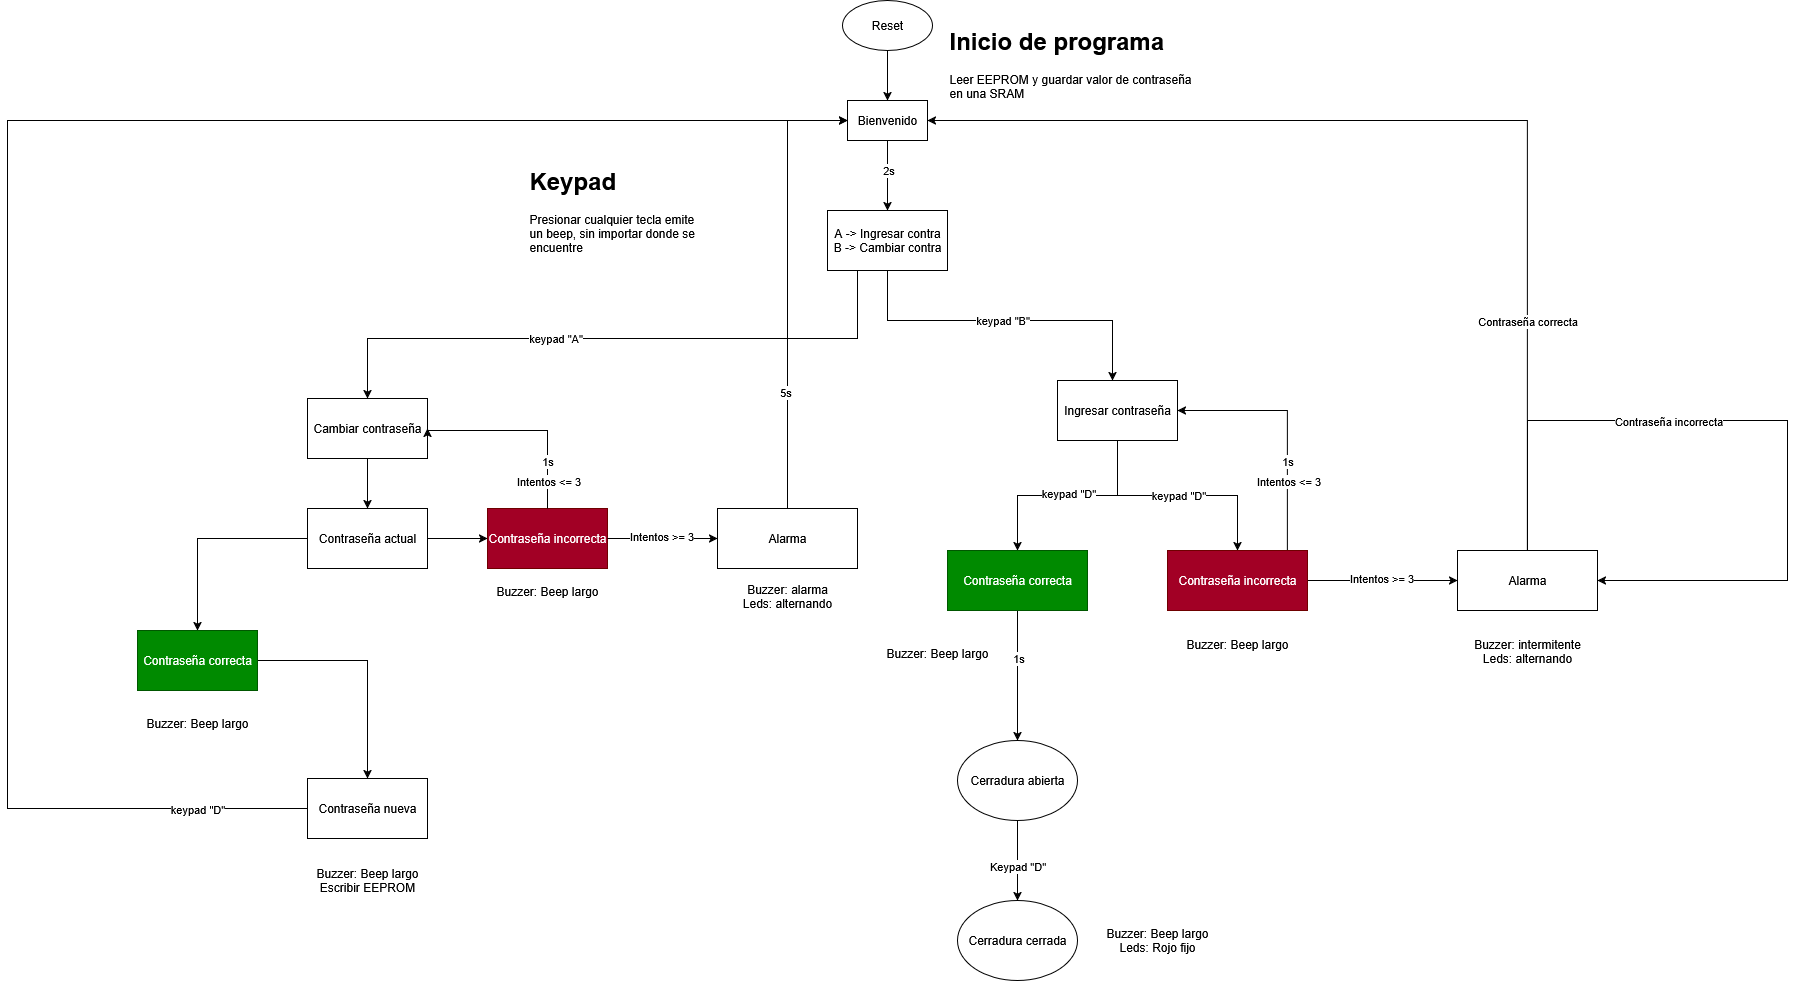
\includegraphics[width=0.9\columnwidth]{anexos/cerradura/DiagramaFlujo.png}
        \caption{Diagrama de flujo de programa de cerradura. Fuente: elaboración própia}
        \label{fig:lcd_ui}
    \end{figure}

    \vspace{1em}
    \paragraph*{\textbf{Interfaz de usuario}}---
    La cerradura dispone de una interfaz de usuario compuesta por una pantalla LCD de 16x2, un teclado matricial 4x4 y tres indicadores luminosos (LED verde, LED rojo y alarma sonora). En este contexto, la interfaz constituye el medio de comunicación entre el usuario y el sistema, mostrando mensajes informativos y recibiendo acciones por medio del teclado. Cada interacción del usuario genera una respuesta visual o acústica distinta, representando así un flujo de diálogo entre ambos.

    \vspace{1em}

    El sistema se diseñó siguiendo una lógica de \textit{máquina de estados finitos}, en la que cada modo de operación (menú principal, ingreso de contraseña, cambio de clave, acceso autorizado, alarma, etc.) representa un estado. Las transiciones entre estados se producen en función de las acciones del usuario y las condiciones del sistema. Este enfoque facilita la gestión de comportamientos complejos, simplifica el control del flujo de ejecución y mejora la legibilidad del código.

    \vspace{1em}
    \paragraph*{\textbf{Teclado matricial}}---
    El ingreso de datos se realiza mediante un teclado matricial 4x4 que combina filas y columnas, optimizando el uso de pines del microcontrolador. Las filas se configuran como salidas y las columnas como entradas con resistencias de \textit{pull-up} activadas. El proceso de lectura consiste en activar una fila a nivel bajo (0) mientras las demás permanecen en alto (1); si alguna tecla de esa fila se encuentra presionada, la columna correspondiente cambia a nivel bajo, permitiendo identificar la intersección entre fila y columna.  

    \vspace{1em}

    Cada tecla se asocia a un carácter según su posición dentro de la matriz, lo que permite retornar el valor numérico o simbólico correspondiente. Para evitar falsas detecciones debido al rebote mecánico de los contactos, se aplica una rutina de \textit{debouncing} por software basada en pequeños retardos temporizados.

    \vspace{1em}

    \paragraph*{\textbf{Planificador de tareas}}---
    Durante el funcionamiento, el sistema debe ejecutar múltiples tareas de forma paralela: reproducción de sonidos, manejo de alarmas, parpadeo de LEDs, lectura del teclado y actualización de la pantalla LCD. Sin embargo, el ATmega328P dispone de un número limitado de temporizadores, por lo que no es posible asignar un temporizador independiente a cada tarea.

    \vspace{1em}

    Para resolver esta limitación, se implementó un esquema de ejecución basado en un \textit{planificador de tareas} o \textit{task scheduler} de propósito general. Se utiliza un solo temporizador configurado para generar interrupciones periódicas, incrementando un contador global de 32 bits que actúa como referencia temporal (en milisegundos). Cada tarea compara el tiempo actual con el instante programado de su próxima ejecución, y si se cumple el intervalo, se ejecuta la acción correspondiente. De este modo, múltiples eventos temporizados pueden coexistir sin emplear retardos bloqueantes ni técnicas de \textit{polling}.

    \vspace{1em}

    Para asegurar que la contraseña permanezca almacenada tras un apagado, se utiliza la memoria EEPROM interna del ATmega328P. Esta memoria no volátil permite conservar los datos durante décadas sin alimentación eléctrica, aunque posee un número limitado de ciclos de escritura (aproximadamente $10^5$ operaciones por celda). Por ello, el sistema únicamente escribe en EEPROM cuando el usuario confirma un cambio de contraseña, minimizando el desgaste de la memoria.

    \vspace{1em}

    La lectura y escritura se realizan mediante las funciones de la biblioteca estándar \texttt{avr/eeprom.h}, que permiten transferir cadenas de caracteres directamente desde y hacia direcciones específicas de la EEPROM. Así, el sistema recupera la contraseña almacenada al inicio del programa y la compara con la ingresada por el usuario durante la operación normal.

    \vspace{1em}

    En conjunto, la cerradura electrónica combina la interacción mediante teclado y pantalla LCD, la gestión de tareas en tiempo real y el almacenamiento persistente de datos, logrando un sistema confiable y autónomo. El uso de una máquina de estados y un planificador temporal basado en un único temporizador permite controlar de manera eficiente múltiples procesos simultáneos sin bloquear la ejecución principal del programa.

